\documentclass[a4paper,12pt]{article}

% Packages
\usepackage[utf8]{inputenc}
\usepackage[english]{babel}
\usepackage{amsmath}
\usepackage{amssymb}
\usepackage{graphicx}
\usepackage{geometry}
\usepackage{float}
\usepackage{caption}
\usepackage{booktabs}
\usepackage{pdfpages}
\usepackage{hyperref}

% Page layout
\geometry{margin=1in}

% Title and Author
\title{Rakéták, rakéta hajtóművek\\ 2. házifeladat}
\author{Ábrók László Patrik\\ JPWF8N}
\date{2025.05.23.} % Date of submission
%\date{\today}

\begin{document}

% Title Page
\maketitle
%\tableofcontents
\newpage

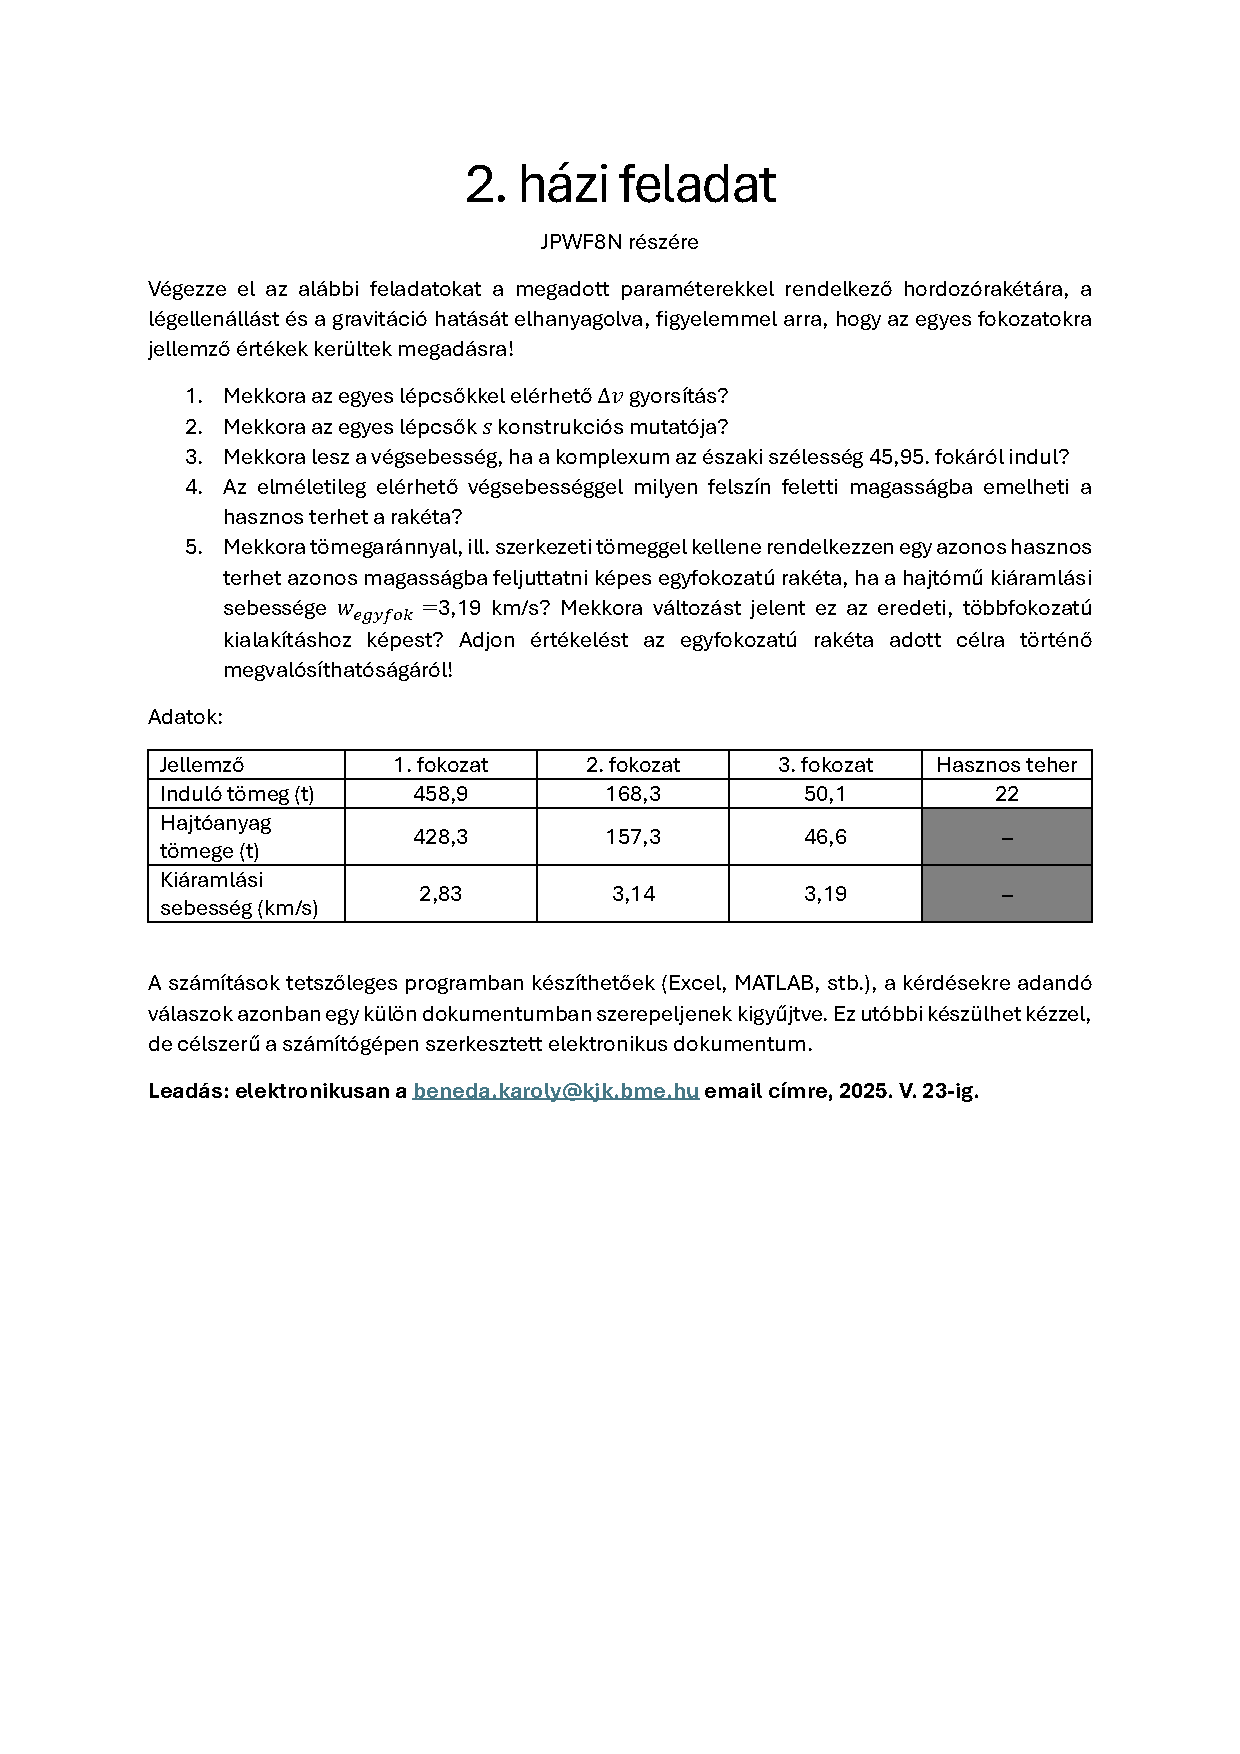
\includepdf[pages=-]{../handout/hw-2-JPWF8N.pdf}

% Section 1: Introduction
\section{Bevezetés}
A feladat elvégzéséhez a Python programozási nyelvet használtam. Az egyes kérdésekhez tartozó számításokat egy Jupyter notebook-ban vezettem le.
A megoldáshoz a következő könyvtárakat használtam:
\begin{itemize}
    \item \texttt{numpy} - numerikus számításokhoz
    \item \texttt{pandas} - adatok kezeléséhez
\end{itemize}
A megoldás megtalálható a következő GitHub repository-ban:
\href{https://github.com/LaszloAbrok/rockets-and-rocket-engines}{rockets-and-rocket-engines repository}

A notebook futtatásához célszerű egy virtuális környezet létrehozása, amelyben a szükséges könyvtárak telepítve vannak.
A szükséges könyvtárak elérhetőek egy requirements.txt fájlban, amelyet a következő paranccsal telepíthetünk:
\begin{verbatim}
pip install -r requirements.txt
\end{verbatim}

Az adatokat két csv fájlban tároltam, amelyet a notebookban beolvasok. A csv fájlok tartalma a következő:
\\
\\
\textbf{data-1.csv}:
\begin{verbatim}
    stage,m_0_t,m_prop_t,vel_out_m_s
    1,458900,428300,2830
    2,168300,157300,3140
    3,50100,46600,3190
\end{verbatim}
\textbf{data-2.csv}:
\begin{verbatim}
    component,m_t
    payload,22000
\end{verbatim}

A feladatleírásban felsorolt mértékegységeket SI-ben adtam meg.

\section{$\Delta$v számítása}

A sebességváltozás kiszámításához Ciolkovszkij egyenletét használtam:

\[
\Delta v_i = w_{e,i} \cdot \ln\left( \frac{m_{0,i}}{m_{f,i}} \right)
\]

\begin{itemize}
    \item \( w_{e,i} \) – az \(i\)-edik fokozat kiáramlási sebessége [m/s],
    \item \( m_{0,i} \) – az \(i\)-edik fokozat induló tömege [kg],
    \item \( m_{f,i} \) – az \(i\)-edik fokozat végső tömege [kg] (felsőbb fokozatok + hasznos teher + saját szerkezet).
  \end{itemize}

Ezáltal a következő értékek adódtak:
\begin{itemize}
    \item Első fokozat: \(\Delta v_1 = 1490.599206 \text{ m/s}\)
    \item Második fokozat: \(\Delta v_2 = 2215.908674 \text{ m/s}\)
    \item Harmadik fokozat: \(\Delta v_3 = 2154.342753 \text{ m/s}\)
\end{itemize}

\section{Konstrukciós mutató}

\[
s_i = \frac{m_{\text{struct},i}}{m_{\text{struct},i} + m_{\text{prop},i}}
\]

ahol:
\begin{itemize}
  \item \( m_{\text{struct},i} \) – az \(i\)-edik fokozat szerkezeti tömege,
  \item \( m_{\text{prop},i} \) – az \(i\)-edik fokozat hajtóanyagtömege.
\end{itemize}

Ebből a következő értékek adódtak:
\begin{itemize}
    \item Első fokozat: \(s_1 = 0.066681\)
    \item Második fokozat: \(s_2 = 0.065359\)
    \item Harmadik fokozat: \(s_3 = 0.069860\)
\end{itemize}

\section{Végsebesség}
\[
v_{\text{final}} = \sum_i \Delta v_i + v_{\text{E}} \cdot \cos(\varphi)
\]

Ahol:
\begin{itemize}
  \item \( \varphi \) – a szélesség (jelen esetben: \(45{,}95^\circ\)),
  \item \( v_{\text{E}} \) – Föld forgási sebessége az egyenlítőnél (kb. 465 m/s).
\end{itemize}

Ebből:
\[
v_{\text{final}} = 6184.158553238991  \text{ m/s}
\]

\section{Maximális magasság}

A következő képpen közelítettem feltételezve azt, hogy elhanyagoljuk a légellenállást és gravitáció változást.

\[
h = \frac{v^2}{2g}
\]

ahol:
\begin{itemize}
  \item \( h \) – magasság [m],
  \item \( v \) – a rakéta végsebessége [m/s],
  \item \( g \) – a nehézségi gyorsulás (\( g \approx 9.81 \, \text{m/s}^2 \)).
\end{itemize}

Innen a magasság:
\[
h = 1949.2261473801716 \text{ km}
\]

\section{Tömegarány és szerkezeti tömeg}

A tömegarányt a következő képlettel számoltam ki:
\[
z = \exp\left(\frac{\Delta v}{w_e}\right)
\]

Ahol:

\[
\Delta v = 5860.8506337930385 \text{ m/s}
\]

és
\[
w_e = 3.191 \text{ km/s}
\]

\[
z = 6.279292104874458
\]

Az induló tömeget pedig a payload és z tömegarány segítségével számoltam ki:

\[
m_0 = z \cdot m_{\text{payload}}
\]

\[
m_0 = 138144.42630723809 \text{ kg}
\]

Előszőr kiszámoltam a három fokozatú rakéta szerkezeti tömegének és üzemanyag tömegének arányát, amelyet a következő képlettel számoltam ki:

\[
r = \frac{m_{\text{struct,3fok}}}{m_{\text{prop,3fok}}}
\]

\[
r = 0.0713381841189497
\]

Ezután az egyfokozatú rakéta hajtóanyag tömege az alábbi képlettel számolható:

\[
m_{\text{prop}} = \frac{m_0 - m_{\text{payload}}}{1 + r}
\]

\[
m_{\text{prop}} = 108410.6102339228 \text{ kg}
\]

A szerkezeti tömeget az induló tömeg, a hasznos teher és a propellánsúly kölönbségeként számítottam:

\[
m_{\text{struct}} = m_0 - m_{\text{payload}} - m_{\text{prop}}
\]

\[
m_{\text{struct}} = 7733.816073315291 \text{ kg}
\]

Az egyfokozatú és háromfokozatú rakéta tömegének aránya:

\[
\text{ratio} = \frac{m_{\text{struct}}}{m_{\text{struct,3fok}}}
\]

\[
\text{ratio} = 0.17148150938614837
\]

Ahol:

\[
m_{\text{struct}} = 45100 \text{ kg}
\]

Az egyfokozatú rakéta a számítások alapján összesen ~7733.82 kg szerkezeti tömeggel rendelkezik, míg a háromfokozatú rakéta 45100 kg szerkezeti tömeggel bír.
A kettő szerkezeti tömegének aránya ~0.1715. Az eredeti háromfokozatúhoz képest ez kevesebb, mint 18\%. Ez azt jelenti, hogy jelentősen csökkenteni kell a szerkezeti tömeget, ahhoz
hogy azonos magasságra juttassuk fel a payload-ot. Egy ilyen rakéta megépítése elméletben lehetséges, de a gyakorlatban sokkal megbízhatóbb megoldás egy több fokozatú rakéta.
\end{document}